\begin{spacing}{1.5}

\section{Resultados experimentales y discusión}\label {sec:results}

\subsection{Materiales utilizados}

La validación experimental se realizó sobre la MIT-BIH Arrhythmia Database \cite{moody2001impact}, disponible públicamente a través de PhysioNet. De los 48 registros que componen la base, se utilizó el registro 100, muestreado a 360 Hz sobre dos derivaciones, del cual se procesó el canal MLII.

La extracción de latidos se apoyó en las anotaciones de referencia del propio registro. De las 2.274 anotaciones disponibles se seleccionaron exclusivamente aquellas etiquetadas como latido sinusal normal (símbolo \texttt{N}), descartando latidos ectópicos, artefactos y marcas de ritmo. Este filtrado produjo un conjunto de 2.237 latidos de las 2.239 anotaciones normales, tras descartar dos: el último latido del registro, que el recorrido de las anotaciones no considera como precaución frente a los bordes, y uno cuya ventana de extracción se salía del registro.

Cada latido se extrajo mediante una ventana \emph{asimétrica} respecto del pico R anotado: 250 ms antes y 500 ms después, es decir 270 muestras a 360 Hz, y se normalizó mediante puntuación Z, de modo que la comparación entre señal real y sintética fuese independiente de la ganancia del canal.

La asimetría se sigue de la fisiología del complejo y no de una conveniencia de implementación. La onda P precede al pico R en unos 150 a 200 ms y dura entre 80 y 110 ms, de modo que su inicio se ubica cerca de 250 ms antes; la onda T termina entre 400 y 450 ms después, dado que el intervalo QT normal ronda los 400 ms. Una ventana centrada en el pico R no puede contener el complejo completo, y la Subsección \ref{sec:validez} cuantifica lo que ocurre cuando se usa una.

El desarrollo se implementó en Python 3.12, empleando NumPy y SciPy \cite{virtanen2020scipy} para el cálculo numérico y la optimización, y WFDB para la lectura de los registros.

\subsection{Diseño de los experimentos}

Para cada uno de los 2.237 latidos se ejecutó un ajuste independiente de los veintidós parámetros del modelo. Veinte de ellos corresponden a la amplitud, la posición temporal y los anchos ascendente y descendente de las cinco Gaussianas asimétricas asociadas a las ondas P, Q, R, S y T. Los dos restantes describen la línea base como un desnivel constante y una tendencia lineal, ambos referidos al instante del pico R, y permiten que el modelo siga el desnivel del segmento ST en lugar de retornar obligadamente a cero entre deflexiones.

La función objetivo minimizada fue el error cuadrático medio (MSE) entre la señal real y la sintética. El ajuste se realizó mediante el algoritmo L-BFGS-B \cite{byrd1995limited}, con restricciones de caja definidas para cada parámetro a partir de rangos fisiológicos, con el propósito de impedir la generación de morfologías biológicamente imposibles.

Las restricciones de amplitud se expresan como fracción del pico del latido y no como valores absolutos en milivoltios. Esta elección no es cosmética. Los latidos ingresan al ajuste normalizados por puntuación Z, de modo que un límite expresado en unidades de la señal cruda deja de tener significado una vez aplicada la normalización. La primera implementación de este trabajo cometió exactamente ese error, y la Subsección \ref{sec:residuo} documenta sus consecuencias y su corrección.

El gradiente de la función objetivo se obtiene de forma analítica a partir de la expresión del modelo, en lugar de estimarse por diferencias finitas, y se entrega directamente al optimizador. La derivación fue verificada contra una aproximación numérica mediante \texttt{scipy.optimize.check\_grad}: sobre cuarenta latidos repartidos a lo largo del registro, evaluada en el punto de partida del optimizador, el error relativo no superó $8{,}9\cdot10^{-6}$. Además de reducir el tiempo de ajuste por latido, esta verificación descarta que las diferencias entre configuraciones del modelo provengan de un gradiente mal estimado.

Conviene precisar la nomenclatura, dado que ambas magnitudes aparecen en la literatura del área: la función objetivo optimizada es el error cuadrático medio (MSE), mientras que la métrica reportada en esta sección es su raíz (RMSE), expresada en unidades de desviación estándar de la señal normalizada. La distinción está impuesta en el propio código: el ajuste persiste ambos valores por separado y la rutina de validación recalcula el RMSE desde las señales reconstruidas, sin reutilizar el valor de la función objetivo. Ese recálculo independiente es lo que permitió detectar, en la primera iteración, que la figura de validación rotulaba como RMSE una cantidad que era MSE.

La evaluación de fidelidad se efectuó comparando cada señal sintética con el latido real que le dio origen, mediante dos métricas complementarias: el coeficiente de correlación de Pearson, que cuantifica la concordancia morfológica, y el RMSE, que cuantifica la discrepancia en amplitud punto a punto.

\subsection{Fidelidad morfológica de las señales generadas}

El Cuadro \ref{tab:metricas} resume el desempeño del generador sobre los 2.237 latidos procesados.

\begin{table}[H]
\centering
\begin{tabular}{|l|c|c|}
\hline
\textbf{Estadístico} & \textbf{Correlación de Pearson} & \textbf{RMSE} \\ \hline
Media & 0,9969 & 0,0779 \\ \hline
Desviación estándar & 0,0015 & 0,0148 \\ \hline
Mínimo & 0,9571 & 0,0466 \\ \hline
Mediana & 0,9971 & 0,0758 \\ \hline
Máximo & 0,9989 & 0,2916 \\ \hline
\end{tabular}
\caption{Métricas de fidelidad del modelo de veintidós parámetros sobre 2.237 latidos normales del registro 100 de MIT-BIH, con la ventana asimétrica de 750 ms.}
\label{tab:metricas}
\end{table}

La correlación media alcanzada fue de 0,9969 con una desviación estándar de 0,0015, y el RMSE medio de 0,0779 desviaciones estándar de la señal normalizada con una desviación de 0,0148. La dispersión reducida de ambas métricas indica que el desempeño es estable a lo largo del registro y no depende de latidos particularmente favorables: la totalidad de los latidos supera una correlación de 0,95, el 99,7\% supera 0,99, ninguno queda por debajo de 0,90, y el 94,1\% presenta un RMSE inferior a 0,10. El peor latido del registro alcanza aun así una correlación de 0,9571. El sesgo medio del residuo fue de $-0{,}0000$ con desviación estándar de 0,0004, es decir indistinguible de cero: el modelo no deja componente sistemática sin explicar.

Corresponde una advertencia sobre la comparación con la iteración anterior de este modelo, que sobre una ventana centrada de 356 ms reportaba una correlación de 0,9986 y un RMSE de 0,0496. Esas cifras \emph{no son comparables} con las de aquí. La ventana pasó de 356 a 750 ms, de modo que hay más del doble de señal que explicar con el mismo número de parámetros, y un error mayor sobre una ventana mayor no indica un modelo peor. Lo que sí es comparable entre ambas versiones, y lo que se reporta a continuación, es la validez de los parámetros ajustados.

El Cuadro \ref{tab:iteraciones} contrasta ambas iteraciones del modelo sobre el mismo conjunto de latidos. La primera es la implementación de veinte parámetros con restricciones expresadas en unidades de señal cruda; la segunda incorpora el término de línea base y expresa las restricciones de amplitud como fracción del pico del latido.

\begin{table}[H]
\centering
\begin{tabular}{|p{5.2cm}|c|c|c|}
\hline
\textbf{Indicador} & \textbf{Primera} & \textbf{Segunda} & \textbf{Tercera} \\ \hline
Ventana de extracción & 356 ms centrada & 356 ms centrada & 750 ms asimétrica \\ \hline
Restricciones de amplitud & en mV & por fracción & por fracción \\ \hline
Parámetros del modelo & 20 & 22 & 22 \\ \hline
Correlación de Pearson & 0,9647 & 0,9986 & 0,9969 \\ \hline
RMSE & 0,3984 & 0,0496 & 0,0779 \\ \hline
Sesgo medio del residuo (sintética $-$ real) & $+0{,}1457$ & $-0{,}0000$ & $-0{,}0000$ \\ \hline
Parámetros saturados por latido & 11,8 de 20 & 1,8 de 22 & 0,83 de 22 \\ \hline
Latidos con el centro de T fuera de la ventana & 0 de 2.238 & 1.637 de 2.238 & 0 de 2.237 \\ \hline
Asimetría mediana del ancho de P & 1,00 & 7,63 & 1,23 \\ \hline
\end{tabular}
\caption{Contraste entre las tres iteraciones del modelo. Las columnas de RMSE no son comparables entre la segunda y la tercera, porque las ventanas abarcan cantidades distintas de señal; las filas de validez de parámetros sí lo son. En la primera iteración, el centro de T y la asimetría de P no delatan el problema porque sus propias cotas los forzaban a valores aceptables: sus parámetros eran artefactos de las restricciones, no del recorte. La primera y la tercera se reproducen con el código actual por línea de comandos; la segunda se re-valida desde sus parámetros guardados.}
\label{tab:iteraciones}
\end{table}

La Figura \ref{fig:validacion} presenta la comparación entre un latido real y su reconstrucción sintética para el caso de mejor ajuste.

\begin{figure}[H]
\centering
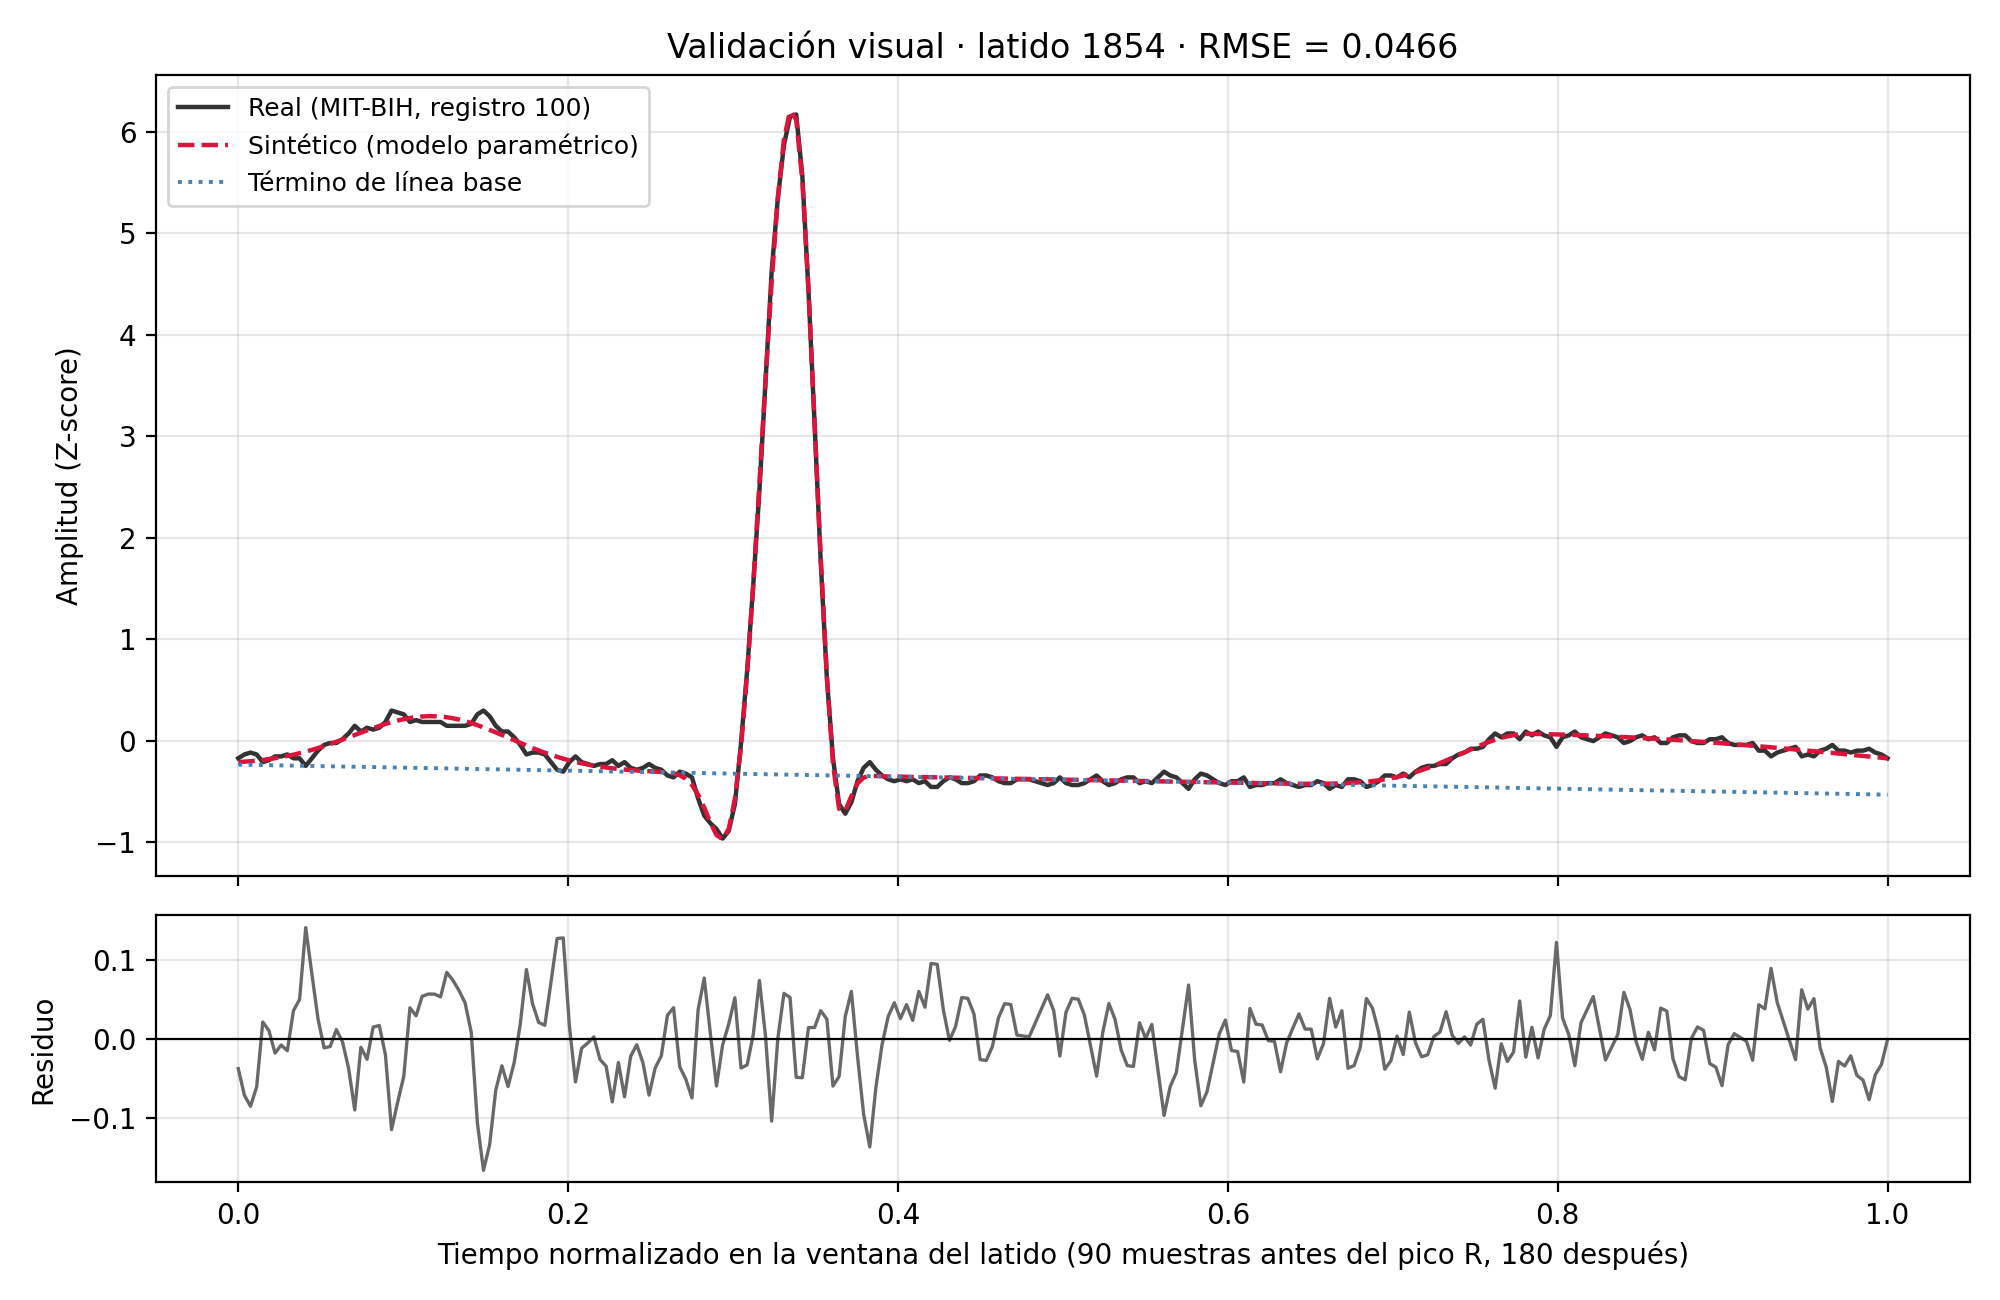
\includegraphics[width=0.95\textwidth]{fig/validacion_visual_v2.png}
\caption{Latido de mejor ajuste del registro 100 bajo la ventana asimétrica de 750 ms: latido 1854, con un RMSE de 0,0466, el mínimo del Cuadro \ref{tab:metricas}. La línea continua es el latido real, la discontinua el modelo ajustado, la punteada el término de línea base, y el panel inferior el residuo punto a punto. Los centros de las cinco ondas quedan dentro de la ventana; la rama descendente de la onda T, en cambio, no alcanza a volver a la línea base antes del borde derecho, que es la limitación que se discute en la Subsección \ref{sec:validez}.}
\label{fig:validacion}
\end{figure}

\subsection{Análisis del error residual y corrección del modelo}\label{sec:residuo}

La primera iteración del modelo, de veinte parámetros, alcanzó una correlación de Pearson media de 0,9647 y un RMSE medio de 0,3984. La lectura conjunta de ambas métricas exigía cautela: esa combinación no describe una reconstrucción de alta fidelidad en sentido estricto, sino un modelo que reproduce correctamente la \emph{forma} del ciclo P-QRS-T conservando una discrepancia de amplitud cercana a 0,4 desviaciones estándar de la señal normalizada. La correlación de Pearson es invariante ante transformaciones afines, de modo que un desplazamiento o un cambio de escala sistemáticos no la penalizan, mientras que sí penalizan el RMSE. Reportar únicamente la correlación habría sobreestimado el desempeño del generador.

El diagnóstico se apoyó en dos instrumentos distintos de la métrica agregada: el conteo de parámetros que convergen exactamente sobre un borde de su restricción de caja, y el sesgo medio del residuo. Un parámetro saturado indica que su valor quedó determinado por el límite y no por los datos; un sesgo no nulo indica una componente del error que el modelo no puede representar por construcción. Ambos instrumentos señalaron una causa concreta.

En primer lugar, se detectó una saturación sistemática en el límite superior del parámetro de amplitud de la onda R. Dicho límite estaba fijado en 3,5 unidades, y 2.234 de los 2.238 latidos (99,8\%) convergieron exactamente sobre esa cota. La causa de fondo es una inconsistencia de unidades: los límites de amplitud fueron derivados de rangos fisiológicos expresados en milivoltios, mientras que los latidos ingresan al ajuste normalizados por puntuación Z, donde el pico R del registro 100 alcanza 5,24 unidades. La restricción de caja, concebida para evitar artefactos, impedía reconstruir la deflexión de mayor amplitud del complejo.

La revisión completa del conteo de saturación mostró que el problema excedía a la onda R. En promedio, 11,8 de los 20 parámetros de cada latido quedaban fijados por un límite, y tres de ellos —el ancho ascendente de Q, el ancho descendente de S y el ancho descendente de T— saturaban en el 100\% de los latidos. El modelo no estaba siendo ajustado a los datos en más de la mitad de sus grados de libertad.

En segundo lugar, se verificó un sesgo sistemático entre ambas señales. El residuo medio, señal sintética menos real, fue de $+0{,}1457$ unidades normalizadas, atribuible a que el modelo de cinco Gaussianas carece de un término de línea base y retorna necesariamente a cero fuera de las deflexiones, mientras que la señal real presenta un desnivel en el segmento ST. Corregir por separado ese desplazamiento constante habría reducido el RMSE medio de 0,3984 a 0,3696, esto es, un 7,2\% del error total, lo que permitía concluir que el sesgo de línea base contribuía sin ser la causa principal del residuo. Esa conclusión resultó correcta: la causa principal era la inconsistencia de unidades en las restricciones de amplitud.

Se aplicaron ambas correcciones. El término de línea base se incorporó como dos parámetros adicionales del modelo, en lugar de restarse a posteriori, de modo que el optimizador lo ajusta simultáneamente con la morfología. Las restricciones de amplitud pasaron a expresarse como fracción del pico del latido. El Cuadro \ref{tab:ablacion} desagrega el aporte de cada corrección.

\begin{table}[H]
\centering
\begin{tabular}{|p{7.6cm}|c|c|}
\hline
\textbf{Configuración del modelo} & \textbf{Pearson} & \textbf{RMSE} \\ \hline
Primera iteración: 20 parámetros, restricciones en unidades de señal cruda & 0,9647 & 0,3984 \\ \hline
Se incorpora el término de línea base (22 parámetros) & 0,9763 & 0,3052 \\ \hline
Se corrigen las restricciones de amplitud, sin línea base (20 parámetros) & 0,9809 & 0,2285 \\ \hline
Ambas correcciones (22 parámetros) & 0,9986 & 0,0496 \\ \hline
\end{tabular}
\caption{Aporte de cada corrección, medido sobre los 2.238 latidos del registro 100. Cada fila corresponde a una corrida completa e independiente del ajuste, reproducible seleccionando el conjunto de restricciones y la presencia del término de línea base por línea de comandos.}
\label{tab:ablacion}
\end{table}

Cada corrección, por separado, mejora el error de forma modesta: la línea base lo reduce un 23,4\% y las restricciones corregidas un 42,7\%. Aplicadas juntas lo reducen un 87,6\%. El efecto conjunto no es, por lo tanto, la suma de los efectos individuales, y la razón es identificable. Mientras la amplitud de la onda R permanece fijada por su límite, el término de línea base absorbe parte del error de amplitud que corresponde a esa onda; y mientras no existe término de línea base, la amplitud liberada de R debe compensar el desnivel del segmento ST. Cada corrección despliega su efecto solo cuando la otra está presente, lo que explica que ninguna de las dos, por separado, anticipara la magnitud de la mejora conjunta.

Tras ambas correcciones el sesgo del residuo es nulo dentro de la precisión de la medición y el promedio de parámetros fijados por un límite cae de 11,8 de 20 a 1,8 de 22.

\subsection{Efecto de la redefinición de la ventana}
\label{sec:validez}

La limitación identificada en la iteración anterior era el largo de la ventana, y su corrección constituye el resultado más claro de esta etapa. Con la ventana centrada de 356 ms, el pico de la onda T caía fuera del recorte en 1.637 de los 2.238 latidos, con una posición mediana 98 ms más allá del borde, y la onda P ajustada presentaba una razón mediana de 7,63 entre sus anchos de subida y de bajada, con un máximo de 30. Una onda que sube siete veces más lento de lo que baja no es una onda P: es el resultado de ajustar una gaussiana contra un flanco parcial. Los parámetros de P y T de esa iteración eran, en consecuencia, artefactos del recorte y no descripciones morfológicas.

Con la ventana asimétrica de 750 ms, las cinco ondas caen dentro del recorte en los 2.237 latidos, y los centros ajustados medianos resultan $-159$ ms para P, $-24$ ms para Q, $+2$ ms para R, $+14$ ms para S y $+339$ ms para T, valores compatibles con la descripción clínica del complejo. La asimetría mediana del ancho de la onda P desciende de 7,63 a 1,23, y el promedio de parámetros determinados por una cota cae de 11,8 de 20 a 0,83 de 22.

\begin{figure}[H]
\centering
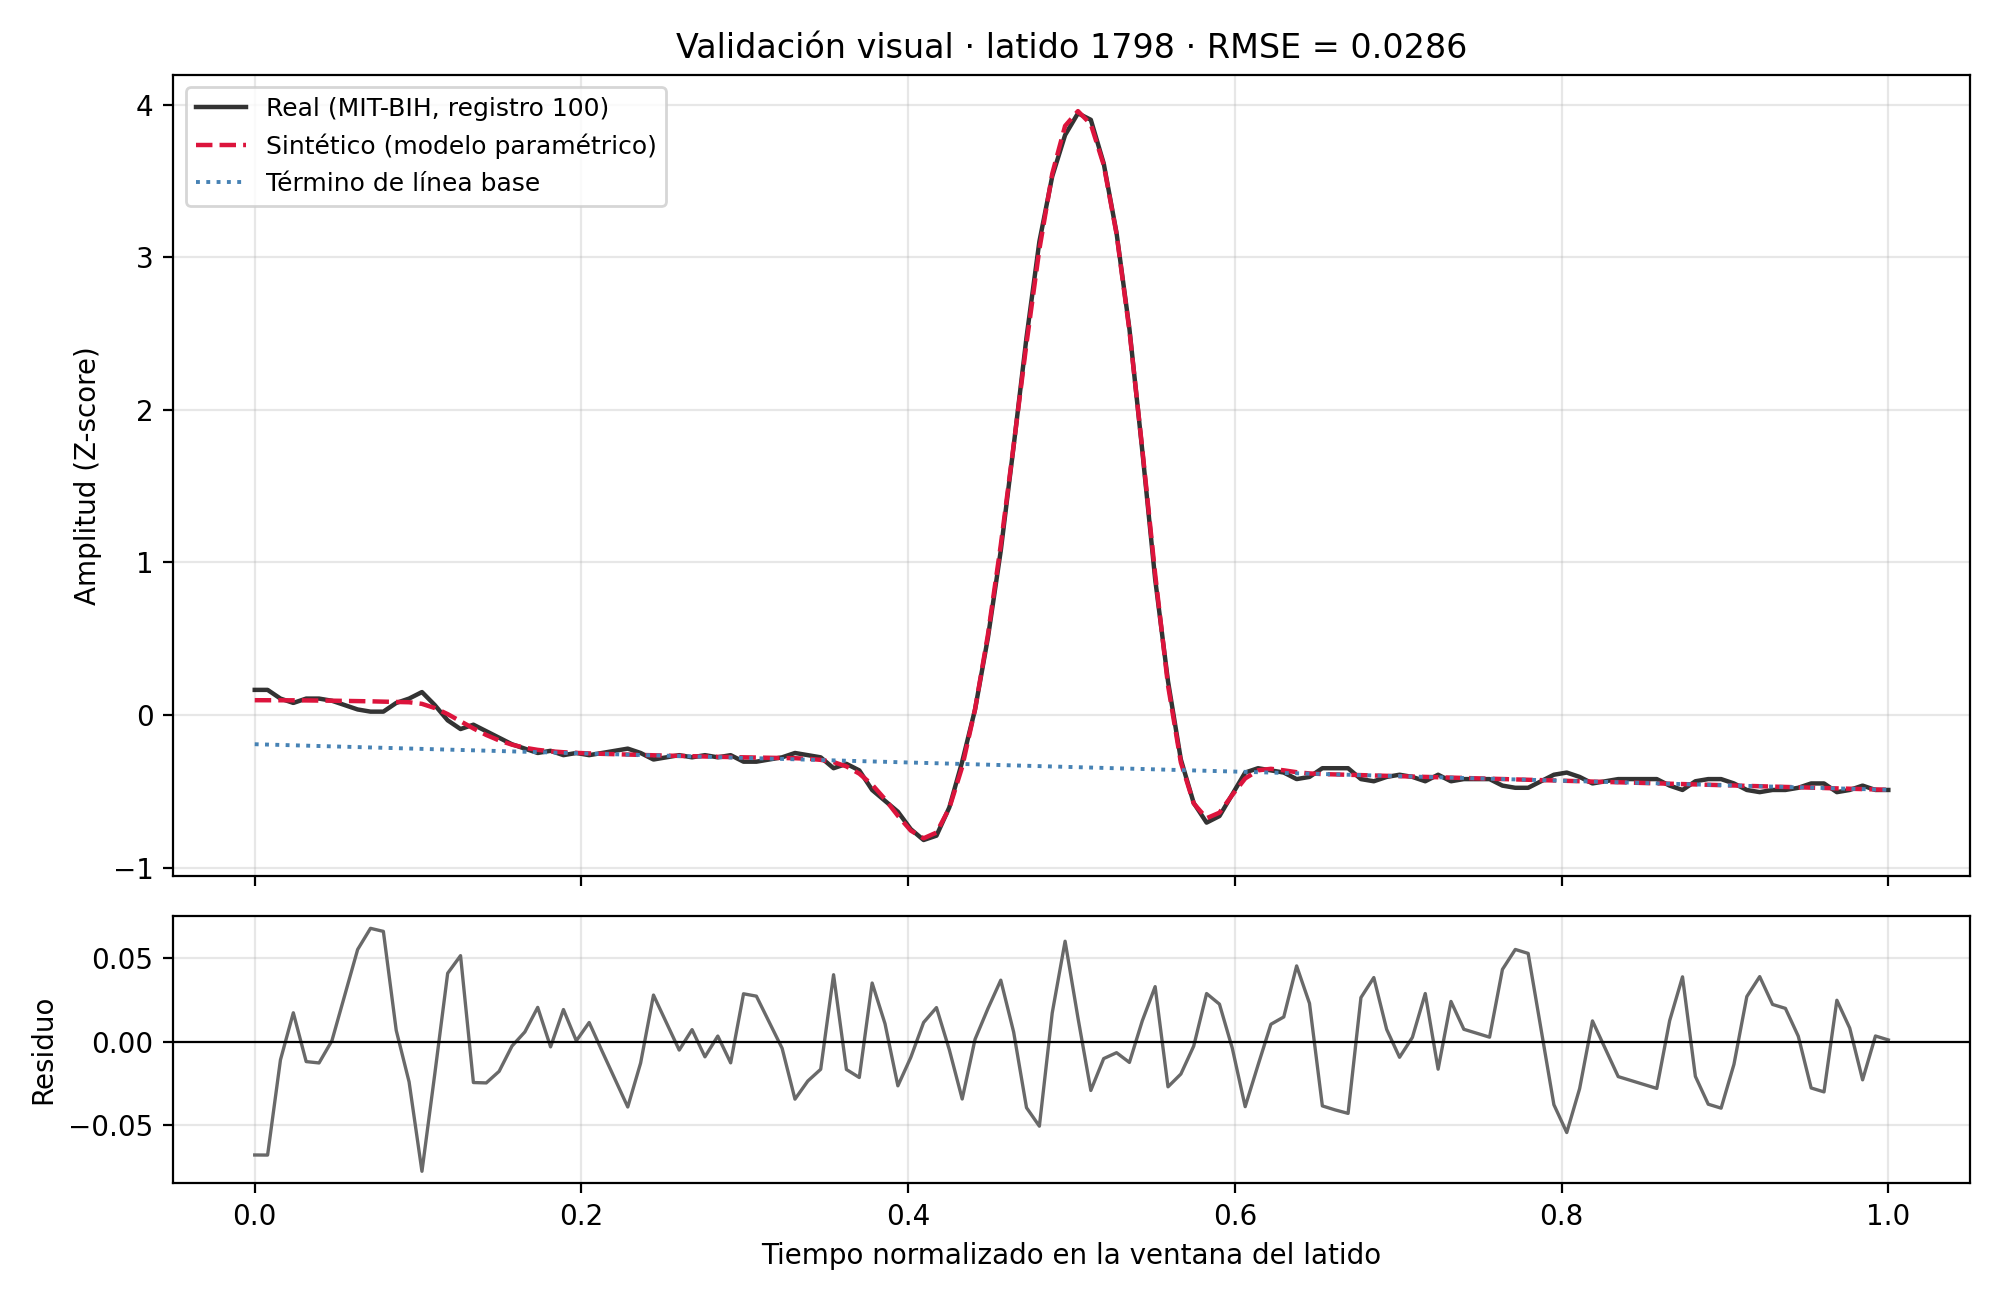
\includegraphics[width=0.85\textwidth]{fig/validacion_visual.png}
\caption{Latido de mejor ajuste de la segunda iteración, con la ventana centrada de 356 ms: latido 1798, RMSE de 0,0286. El recorte deja fuera el inicio de la onda P por la izquierda y la onda T por la derecha, de modo que el modelo ajusta sus gaussianas contra flancos incompletos. Su RMSE no es comparable con el de la Figura \ref{fig:validacion}, porque la ventana contiene menos de la mitad de la señal. Compárese con la Figura \ref{fig:validacion}, que muestra el mismo registro bajo la ventana asimétrica.}
\label{fig:validacion_v2}
\end{figure}

\subsubsection{Limitación remanente: la forma de la onda T}

La saturación no desaparece por completo. Un parámetro concentra prácticamente toda la que queda: el ancho de la rama descendente de la onda T converge sobre su cota de 180 ms en el 71,9\% de los latidos.

Se puso a prueba la hipótesis de que esa gaussiana estaba absorbiendo una deriva que la línea base afín no podía seguir a lo largo de 750 ms, agregando un término cuadrático de línea base como parámetro veintitrés, con el gradiente analítico extendido y verificado contra diferencias finitas. La hipótesis queda \emph{rechazada}: el RMSE mejora apenas un 2,3\%, de 0,0781 a 0,0763, y la saturación cae solo de 25 a 22 latidos de 40. Aflojar la cota produce un resultado análogo: con un tope de 300 ms el ajuste elige 232 ms y el error mejora un 2,7\%, y con un tope de 600 ms elige el mismo valor, de modo que es el dato y no la cota quien lo fija. Pero un ancho de 232 ms no describe una onda T, cuya duración total ronda los 160 ms: describe una deriva.

Se puso a prueba también la opción de representar la onda T con \emph{dos} gaussianas en lugar de una, llevando el modelo a veintiséis parámetros, con los centros ordenados por rango para que las dos componentes no fuesen intercambiables y con el gradiente analítico correspondiente verificado. Sobre cuarenta latidos, el RMSE mejora un 6,8\%, de 0,0776 a 0,0724, y el criterio de información bayesiano, que penaliza el número de parámetros, favorece al modelo de veintiséis por 15,4 unidades, una diferencia que se considera decisiva. Por ajuste, la segunda gaussiana se justifica. Pero la saturación, que era el problema a resolver, \emph{aumenta}: el promedio de parámetros determinados por una cota sube de 0,68 a 1,50 por latido, y la rama descendente de la última gaussiana de T pasa de saturar en 26 a saturar en 33 latidos de 40. El modelo de veintiséis parámetros ajusta mejor la señal, pero lo consigue con más parámetros cuyo valor fija el borde del dominio y no los datos, que es precisamente la condición que el control de saturación de la Sección \ref{sec:mp} declara invalidante para la interpretación fisiológica de un parámetro.

Ninguna de las tres hipótesis puestas a prueba —el término cuadrático de línea base, el aflojamiento de la cota y la segunda gaussiana— resuelve la saturación de la rama descendente de la onda T: las dos primeras apenas mejoran el error, y la tercera lo mejora a costa de aumentarla. La conclusión que sostiene la evidencia es, por lo tanto, más acotada que un rechazo: dentro de esta familia de funciones, la mejora de ajuste disponible se obtiene sacrificando la interpretabilidad de los parámetros, que es la propiedad que justifica un modelo paramétrico frente a uno de caja negra. Este trabajo conserva el modelo de veintidós parámetros por esa razón, y no porque el de veintiséis ajuste peor. La explicación remanente, visible en la Figura \ref{fig:validacion}, es que la onda T de este registro presenta una meseta ancha y no una campana, y una suma de gaussianas asimétricas no representa un plateau con parsimonia. La limitación se declara como tal, ahora acotada por medición y no por conjetura: corresponde explorar otra familia de funciones para la repolarización, y no ampliar la actual.

Vale registrar un detalle metodológico de esa prueba. Un primer intento, realizado sin gradiente analítico, produjo un RMSE \emph{peor} con \emph{más} parámetros, lo cual es imposible en un modelo anidado y por lo tanto delataba falta de convergencia y no una propiedad del modelo. Sin ese chequeo de coherencia se habría concluido lo contrario de lo correcto.

\subsection{Módulo de ritmo: recuperación del exponente prescrito}

Las secciones anteriores evalúan la forma del latido. Esta evalúa el tiempo
entre latidos, que es el aporte de esta versión del trabajo, y lo hace con un
criterio distinto: en lugar de preguntar si la serie generada se parece a una
real, se pregunta si posee la propiedad que se le pidió.

\subsubsection{Verificación del generador contra su propio estimador}

El primer control consiste en comprobar que la relación
$\alpha = (\beta+1)/2$ se cumple en la implementación. Sobre series de 32.768
puntos y doscientas realizaciones independientes por valor, el sesgo del
exponente recuperado no supera 0,011 en valor absoluto para $\alpha$ entre 0,6
y 1,4. Esto verifica el par generador-estimador de manera conjunta: un error en
cualquiera de los dos aparecería como una discrepancia sistemática mayor.

\subsubsection{Sesgo del estimador según el largo del registro}

El Cuadro \ref{tab:sesgo} reporta el exponente recuperado en función del
exponente pedido y del largo de la serie. Este cuadro no es un accesorio: es la
condición para poder interpretar un exponente medido sobre datos reales. El
sesgo es negativo, tiende a crecer con $\alpha$ y decrece con el largo del
registro, de modo que sin caracterizarlo no hay forma de distinguir un
exponente fisiológico de un artefacto de un registro corto.

\begin{table}[H]
\centering
\begin{tabular}{|c|c|c|c|}
\hline
\textbf{$\alpha$ pedido} & \textbf{$N=512$} & \textbf{$N=4.096$} & \textbf{$N=32.768$} \\ \hline
0,6 & $0{,}592 \pm 0{,}073$ & $0{,}593 \pm 0{,}030$ & $0{,}597 \pm 0{,}018$ \\ \hline
0,8 & $0{,}785 \pm 0{,}079$ & $0{,}792 \pm 0{,}037$ & $0{,}794 \pm 0{,}021$ \\ \hline
1,0 & $0{,}974 \pm 0{,}093$ & $0{,}986 \pm 0{,}040$ & $0{,}995 \pm 0{,}020$ \\ \hline
1,2 & $1{,}174 \pm 0{,}104$ & $1{,}184 \pm 0{,}044$ & $1{,}189 \pm 0{,}027$ \\ \hline
1,4 & $1{,}366 \pm 0{,}105$ & $1{,}383 \pm 0{,}048$ & $1{,}391 \pm 0{,}028$ \\ \hline
\end{tabular}
\caption{Exponente recuperado de la serie generada, como media $\pm$ desviación estándar sobre doscientas realizaciones independientes por celda; el error estándar del sesgo no supera 0,008. El sesgo del estimador es negativo, tiende a crecer con el exponente y decrece con el largo del registro.}
\label{tab:sesgo}
\end{table}

\subsubsection{Cohorte sintética de veinticuatro horas}

Se generó una cohorte de cincuenta sujetos sintéticos de veinticuatro horas cada
uno, con 101.647 latidos por sujeto y un exponente sorteado por sujeto de una
distribución normal, de modo que la cohorte tenga dispersión entre individuos y
no un único exponente repetido. La correlación entre el exponente pedido y el
recuperado es de 0,98, con un error absoluto medio de 0,014, y ningún intervalo
requirió recorte por salirse del rango fisiológico. El exponente de corto
alcance de la cohorte resultó $\alpha_1 = 1{,}17 \pm 0{,}09$, unas tres
centésimas por encima del exponente global recuperado, $1{,}14$. Esa diferencia
no debe leerse como un cruce de pendiente: el generador es monofractal, produce
un único exponente en todas las escalas, y el exceso de $\alpha_1$ es
consistente con el sesgo positivo del estimador en ventanas de pocos latidos
descrito en la Sección \ref{sec:mp}. Tampoco debe leerse como una validación
frente al valor de 1,17 reportado para adultos sanos
\cite{costa2017fragmentation}: el exponente que se le pidió a la cohorte se
sorteó de una distribución centrada precisamente en ese valor. Reproducir el
cruce entre $\alpha_1$ y $\alpha_2$ que se observa en sujetos sanos exigiría
un generador con dos regímenes de escalamiento, y queda planteado como
extensión.

\begin{figure}[H]
\centering
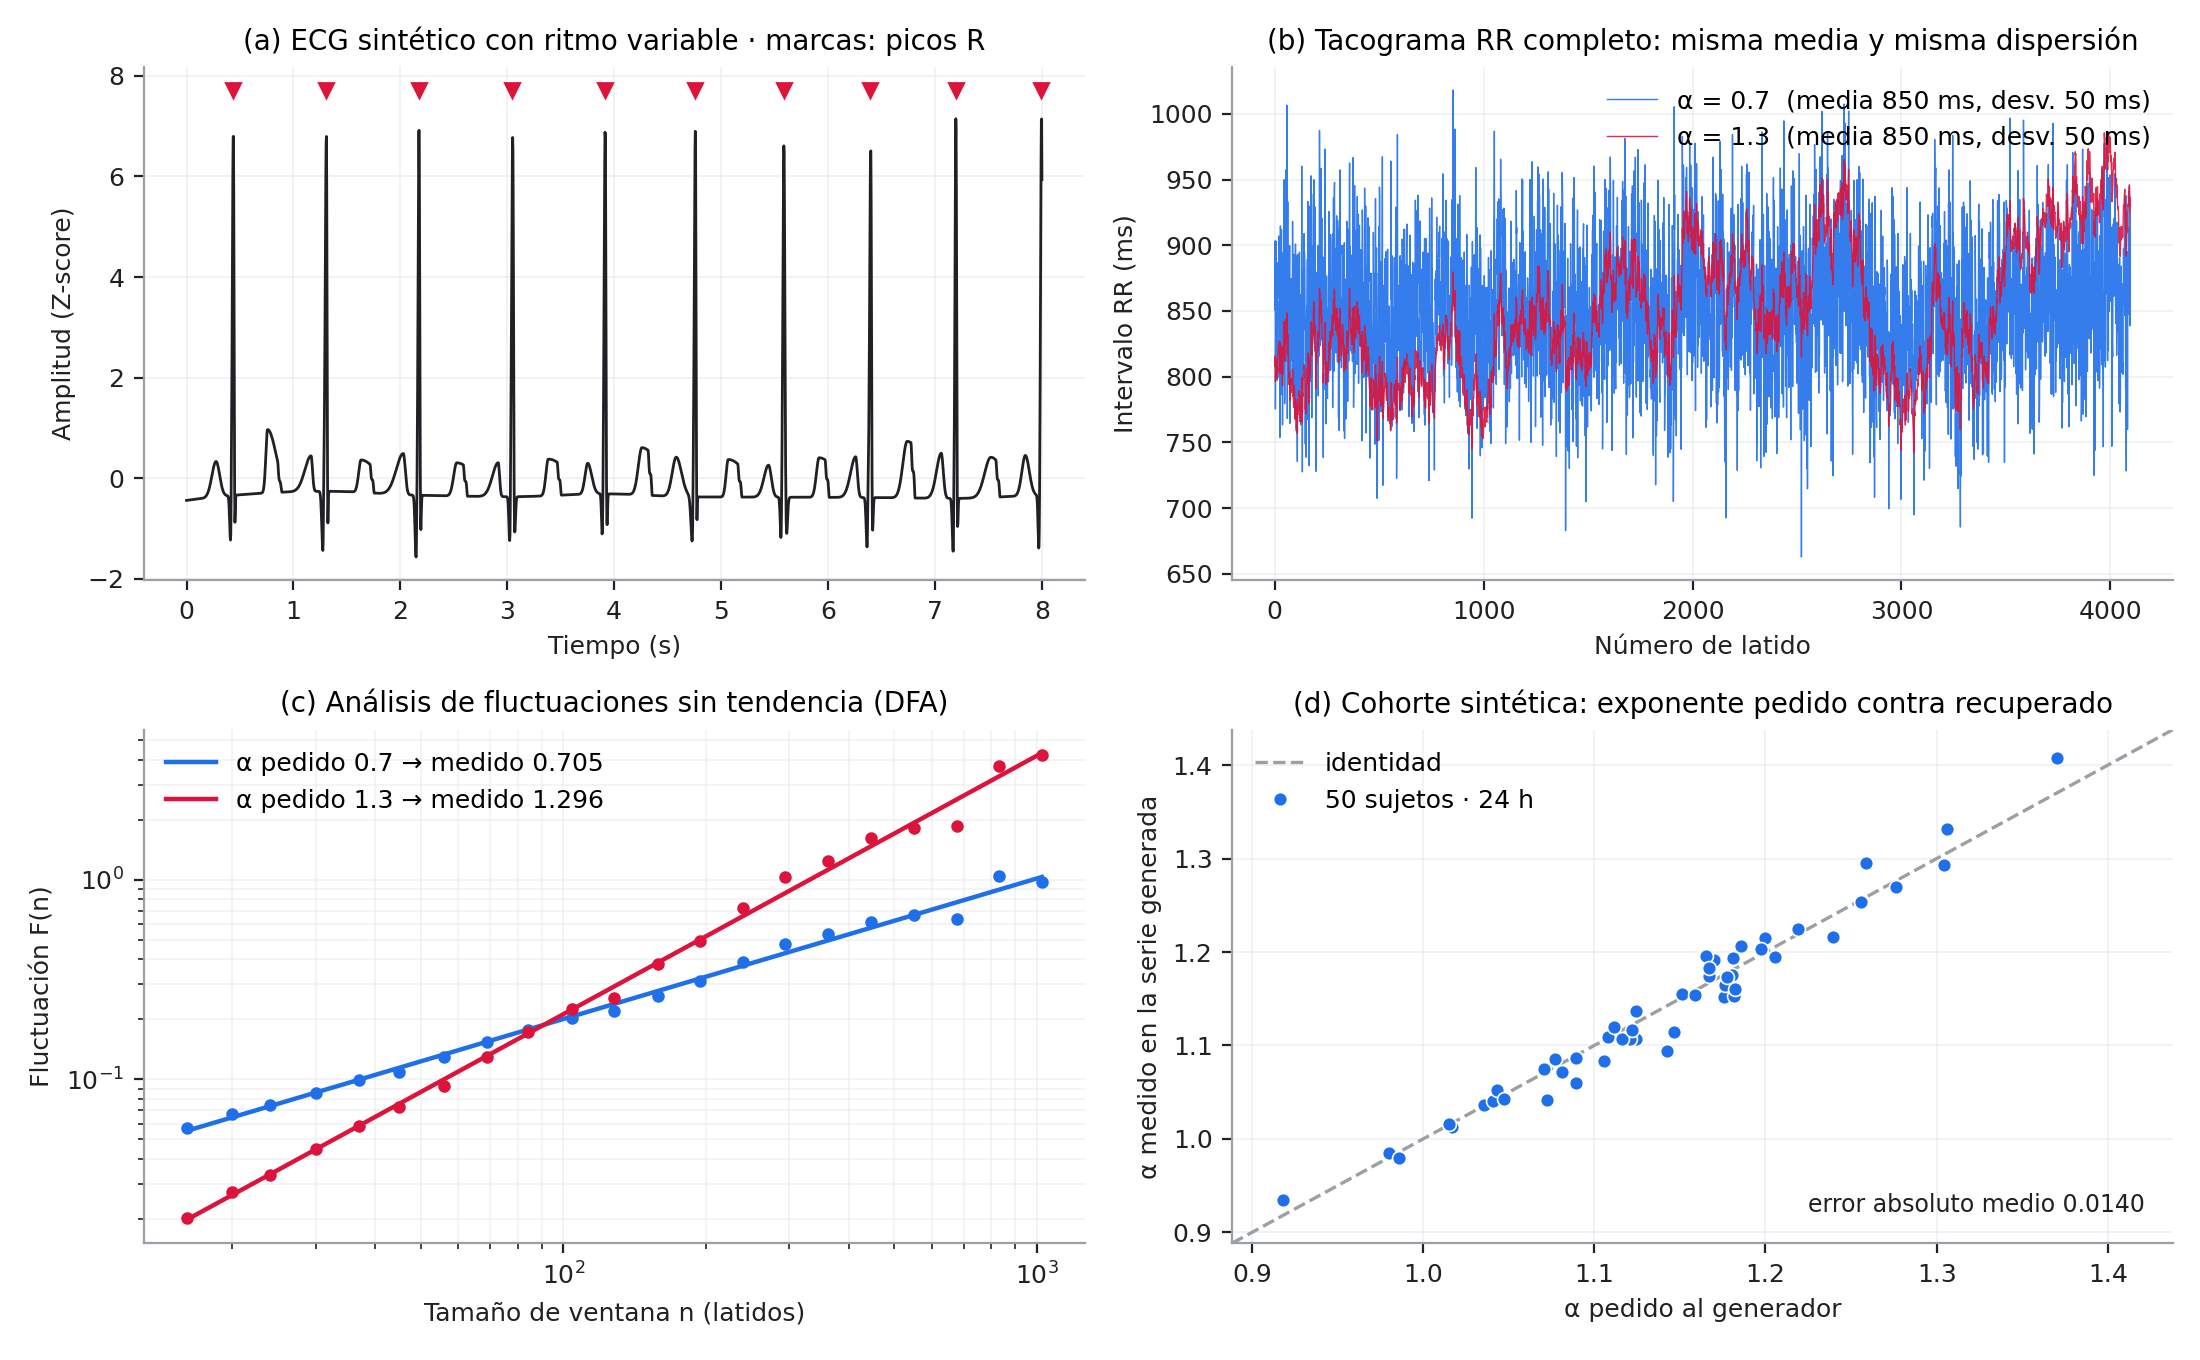
\includegraphics[width=\textwidth]{fig/validacion_hurst.png}
\caption{Validación del módulo de ritmo. (a) Ocho segundos de ECG sintético con ritmo variable; las marcas señalan los picos R. (b) Dos tacogramas R-R con la misma media y la misma desviación estándar pero distinto exponente de escalamiento. (c) Análisis de fluctuaciones sin tendencia de esas dos series, con el exponente pedido y el recuperado. (d) Cohorte de cincuenta sujetos sintéticos de veinticuatro horas: exponente pedido contra exponente recuperado, con la recta identidad como referencia.}
\label{fig:ritmo}
\end{figure}

El panel (b) de la Figura \ref{fig:ritmo} muestra el punto de toda la
construcción. Los dos tacogramas comparten media y desviación estándar, de modo
que cualquier índice convencional de variabilidad en el dominio del tiempo los
reportaría como equivalentes; difieren únicamente en la organización temporal de
sus fluctuaciones, que es la dimensión que el exponente captura y que esos
índices no ven.

\subsection{Motor de reglas fisiológicas: cohorte etiquetada}\label{sec:cohorte}

Se generó una cohorte de 500 sujetos sanos y 500 enfermos con el motor descrito en la Subsección~\ref{sec:reglas}, con semilla 0, sobre la plantilla morfológica de los 2.237 latidos ajustados y en el estrato de referencia de hombres de 60 a 69 años. El archivo de la cohorte registra la semilla, el estrato, el conjunto de parámetros de origen, la geometría de la ventana y el entorno de cálculo, de modo que puede regenerarse exactamente.

El Cuadro~\ref{tab:cohorte} resume la verificación. Ninguna de las cinco condiciones falla en ninguno de los mil sujetos.

\begin{table}[H]
\centering
\begin{tabular}{|p{9cm}|c|}
\hline
\textbf{Condición verificada} & \textbf{Sujetos que la incumplen} \\ \hline
Rasgo impuesto con error mayor a 1 ms & 0 de 1.000 \\ \hline
Sujeto sano con un rasgo impuesto fuera de su rango & 0 de 500 \\ \hline
Sujeto enfermo con su rasgo desviado dentro del rango & 0 de 500 \\ \hline
Onda T solapada con el complejo QRS & 0 de 1.000 \\ \hline
Centro de la onda T fuera de la ventana de extracción & 0 de 1.000 \\ \hline
\end{tabular}
\caption{Verificación de la cohorte de 500 sujetos sanos y 500 enfermos, medida sobre los parámetros efectivamente generados.}
\label{tab:cohorte}
\end{table}

En el grupo de enfermos, el rasgo desviado se distribuyó entre 131 sujetos por el intervalo PR, 132 por la duración del QRS, 130 por el intervalo QT y 107 por la duración de la onda P. En el grupo control, los intervalos medidos cubren los rangos de referencia completos: el PR va de 114,0 a 216,0~ms, el QRS de 76,0 a 113,9~ms y el QT de 338,6 a 471,5~ms. Este último alcanza valores por encima de 450~ms sin que ello constituya un error de etiquetado, por las razones expuestas en la Subsección~\ref{sec:reglas}: se trata de QT sin corregir por frecuencia. El centro de la onda T de los sujetos sanos se ubica entre 122 y 316~ms después del pico R; en ausencia de un rango de referencia para esa posición, la cifra se informa como observación y no como criterio de validez.

\subsection{Alcance efectivo respecto a los resultados proyectados}

Por transparencia metodológica, el Cuadro \ref{tab:alcance} contrasta los resultados proyectados en la propuesta de esta investigación con lo efectivamente alcanzado hasta la fecha.

\begin{table}[H]
\centering
\begin{tabular}{|p{7cm}|p{6.5cm}|}
\hline
\textbf{Resultado proyectado} & \textbf{Estado actual} \\ \hline
Framework de generación paramétrica en Python & Implementado y funcional para latidos sinusales normales \\ \hline
Validación de fidelidad frente a MIT-BIH & Realizada sobre 1 registro de los 48 de la base \\ \hline
Dataset de al menos 5.000 latidos sintéticos & 2.237 latidos parametrizados, más una cohorte de 50 series de 24 horas \\ \hline
Motor de reglas fisiológicas para grupo control y grupo de enfermos & Implementado y verificado sobre una cohorte de 500 sanos y 500 enfermos, en un estrato de referencia fijo \\ \hline
Validación del conjunto sintético con red neuronal preentrenada & No realizada \\ \hline
Publicación en revista indexada & Pendiente \\ \hline
\end{tabular}
\caption{Contraste entre los resultados proyectados y los alcanzados.}
\label{tab:alcance}
\end{table}

El motor de reglas fisiológicas se implementó y verificó con dos restricciones de alcance: opera sobre un único estrato de referencia, sin variar el sexo ni la edad, y construye sus etiquetas solo sobre intervalos morfológicos, sin intervención del exponente de escalamiento del ritmo. La validación del conjunto sintético mediante un modelo preentrenado queda fuera del alcance de esta etapa. En consecuencia, las conclusiones sobre fidelidad morfológica son válidas para ritmo sinusal normal, y las etiquetas del motor describen cómo se construyó cada sujeto, no una condición clínica.

\subsection{Resultados de responsabilidad social}

El proyecto pretende democratizar el acceso a datos médicos de alta calidad sin comprometer la privacidad de los pacientes. Al proporcionar un generador robusto, se facilita que investigadores en regiones con pocos recursos clínicos puedan desarrollar y validar sus propios algoritmos de diagnóstico cardiovascular, promoviendo la equidad en las tecnologías de salud asistida.

\end{spacing}
